\begin{lemma}{Satz über die Umkehrabbildung}
    Sei $I \subseteq \R$ ein Intervall und $f:I \to \R$ stetig, streng monoton. Dann ist $J \coloneqq f(I) \subseteq \R$ ein Intervall und $f^{-1}: J \to I$ ist stetig, streng monoton.
\end{lemma}

\begin{example}
    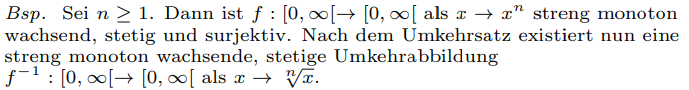
\includegraphics[scale=0.5]{Analysis1/zsf/Images/Stetige_Funktionen/bsp_umkehrabbildung.png}
\end{example}

